\chapter{Ejercicio Servidores Replicados}
En este ejercicio debemos gestionar los registros de los clientes y sus donaciones
entre dos réplicas distintas.

En la clase \texttt{Servidor} tendremos la estructura de este y se instanciarán el
número máximo de réplicas que se desee, con la clase \texttt{Replicas}.

He modificado el código para que el máximo de réplicas sean 4, cuando se intente registrar un nuevo
cliente se procederá de la siguiente forma:

\begin{lstlisting}[language=java]
public int registrarCliente(int id_cliente) throws RemoteException, NotBoundException {
	int rep_min_registrados = id_replica;
	int min_total_registrados = getTotalClientes();
	boolean registrado = false;
	Replicas_I candidata = (Replicas_I) this;

	for (int i = 0; i < Replicas.total_replicas; i++) {
		if (i != this.id_replica) {
			candidata = (Replicas_I) registry.lookup("Replica" + i);

			registrado = candidata.getRegistrado(id_cliente);

			//Buscar la réplica que tiene menor número de clientes registrados
			int total_registrados_candidata = candidata.getTotalClientes();
			if(total_registrados_candidata < min_total_registrados) {
				rep_min_registrados = i;
				min_total_registrados = total_registrados_candidata;
			}
		}
	}

	if(!registrado) {
		if (rep_min_registrados != id_replica) {
			candidata = (Replicas_I) registry.lookup("Replica" + rep_min_registrados);
			candidata.registrarCliente(id_cliente);
		}
		else {
			System.out.println("Cliente " + id_cliente + " registrado en réplica " + this.id_replica);
			this.clientes_registrados.put(id_cliente, 0);
		}
	}

	return rep_min_registrados;
}
\end{lstlisting}

Se escoge la réplica actual como candidata y se cicla entre todas las réplicas que hay en el registro mientras
no estemos buscando la actual. Si en la réplica encontrada hay menos clientes que en la candidata se actualiza
esta para que la réplica i sea la nueva candidata. Una vez acabado el bucle registramos el cliente en la réplica candidata.

Las donaciones de los clientes se guardan en un \texttt{HashMap} donde la clave es el id de cliente y el valor la cantidad total
que ha donado ese cliente, para recuperar el total donado guardado entre todas las réplicas se vuelve a cliclar entre ellas
sumando los subtotales de cada una.

\begin{lstlisting}[language=java]
public int getTotalDonaciones(int id_cliente) throws RemoteException, NotBoundException {
	int total = -1;

	if(getRegistrado(id_cliente) && haDonado(id_cliente)) {
		total = getSubtotalDonaciones();
		for (int i = 0; i < Replicas.total_replicas; i++)
			if(i != id_replica)
				total +=((Replicas_I) registry.lookup("Replica" + i)).getSubtotalDonaciones();
	}

	return total;
}
\end{lstlisting}


Para ejecutar tendremos que usar:

\begin{lstlisting}[language=sh]
	java -cp . -Djava.rmi.server.codebase=file:./ -Djava.rmi.server.hostname=localhost -Djava.security.policy=server.policy practica3.Servidor
	java -cp . -Djava.rmi.server.codebase=file:./ -Djava.rmi.server.hostname=localhost -Djava.security.policy=server.policy practica3.Cliente
\end{lstlisting}

Un ejemplo de ejecución:

\begin{figure}[!ht]
	\begin{center}
		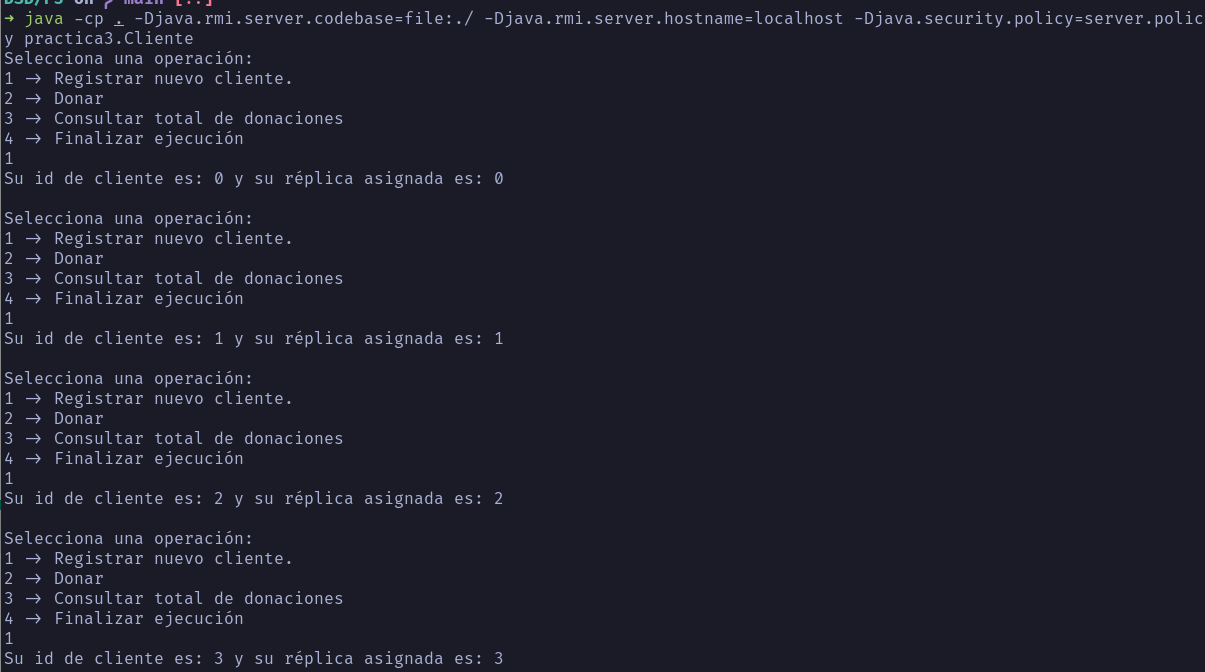
\includegraphics[scale=0.5]{clienteP3.png}
	\end{center}
\end{figure}

\begin{figure}[!ht]
	\begin{center}
		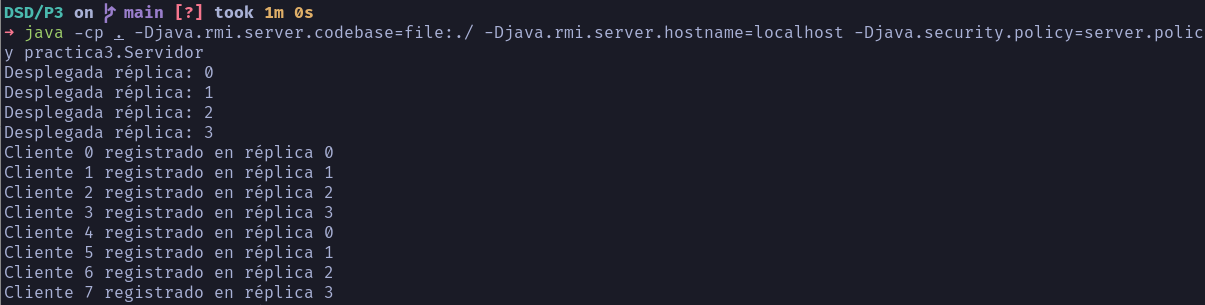
\includegraphics[scale=0.5]{servidorP3.png}
	\end{center}
\end{figure}
